\documentclass[10pt,a4paper]{article}
\usepackage[utf8]{inputenc}
\usepackage{amsmath}
\usepackage{amsfonts}
\usepackage{amssymb}
\usepackage{braket}
\usepackage[ngerman]{babel}
\usepackage{graphicx}
\author{Pascal Bies, Daniel Kosinksi, Patrick Petersen}
\title{Moderne Physik für Informatiker Zusammenfassung}
\begin{document}
\maketitle

\begin{abstract}
Zusammenfassung der "Moderne Physik für Informatiker"'-Vorlesung von Prof. Dr.Schnirman.
\end{abstract}

\setcounter{tocdepth}{3}


\newpage
\tableofcontents


\newpage

\section{Mathe Tricks}

Trigonometrische Funktionen:
\begin{eqnarray}
1=sin^2(x)+cos^2(x)\\
\sin(x+y) = \sin(x)*cos(y) + \cos(x)*sin(y)\\
\sin(x-y) = \sin(x)*cos(y) - \cos(x)*sin(y)\\
\cos(x+y) = \cos(x)*cos(y) - \sin(x)*sin(y)\\
\cos(x-y) = \cos(x)*cos(y) + \sin(x)*sin(y)
\end{eqnarray}
%
\\
Ableitung:
\begin{eqnarray}
\frac{df}{dt} = \frac{d}{dt} f(x(t),y(t),z(t))=  \frac{\partial f}{\partial x} \frac{x}{t} + \frac{\partial f}{\partial y} \frac{y}{t} + \frac{\partial f}{\partial z} \frac{z}{t} + \frac{\partial f}{\partial t}
\end{eqnarray}
%
\\
Kugelkoordinaten:
\begin{eqnarray}
x = r \sin(\theta)cos(\phi)\\
y = r \sin(\theta)sin(\phi)\\
z = r \cos(\theta)\\
\dot{x} =\dot{r}\sin(\theta)\cos(\phi)+r\cos(\theta)\cos(\phi)\dot{\theta }-r\sin(\theta)\sin(\phi)\dot{\phi}\\
\dot{y} = \dot{r}\sin(\theta)\sin(\phi)+r\cos(\theta)\sin(\phi)\dot{\theta }+r\sin(\theta)\cos(\phi)\dot{\phi}\\
\dot{z}= \dot{r}\cos(\theta)-r\sin(\theta)\dot{\theta}
\end{eqnarray}
%
\\
Zylinderkoordinaten:
\begin{eqnarray}
x = \rho \cos(\phi)\\
y = \rho \sin(\phi)\\
z = z
\end{eqnarray}
%
pq formel = $x_{1,2} = - \frac{p}{2}\pm\sqrt{\left(\frac{p}2\right)^2 - q}$\\
%
\\
Komplexezahlen:\\
$|z|=\sqrt{z*z^*}=\sqrt{(a-ib)(a-ib)}=\sqrt{a^2+b^2}$\\
$z*z^*=|z|$\\
%
\\
Eigenvektoren: Bestimme $\lambda$ mit $det(A-\lambda E)=$char-poly. Löse Gleichungen nach 0 und setze in $|a|^2+|b|^2+..... = 1$, falls normiert, andernfalls normieren.\\
%
\\
Determinante von 3x3-Matrix:\\
\begin{align}\det A &= \det \begin{pmatrix} a_{11} & a_{12} & a_{13} \\ a_{21} & a_{22} & a_{23} \\ a_{31} & a_{32} & a_{33} \end{pmatrix}\\ &= a_{11} a_{22} a_{33} +a_{12} a_{23} a_{31} + a_{13} a_{21} a_{32} - a_{13} a_{22} a_{31} - a_{12} a_{21} a_{33} - a_{11} a_{23} a_{32}.\end{align}\\
%
\\
Inverse\\
$A^{-1} = \frac{1}{\det A} \cdot \operatorname{adj} A$\\
$\operatorname{adj} (A) = \begin{pmatrix} \,\,\,{{d}} & \!\!{{-c}}\\ {{-b}} & {{a}} \end{pmatrix} ^T = \begin{pmatrix} \,\,\,{{d}} & \!\!{{-b}}\\ {{-c}} & {{a}} \end{pmatrix}$\\
\begin{align}\operatorname{adj} (A)& =\begin{pmatrix}ei - fh & ch - bi & bf - ce \\fg - di & ai - cg & cd - af \\dh - eg & bg - ah & ae - bd\end{pmatrix}\end{align}


\section{Newtonsche Mechanik}
\subsection{Konservative Kräfte}
$[r,r_0]=\int_{r_0}^r F(r) dr \Rightarrow dw = Fdr$\\
%
\\
$\frac{d}{dt}T=mv\dot{v}=vF \Rightarrow dT = VFdt = Fdr = dW$\\
Spezialfall: $F=-\vec{\nabla}V=\oint Fdr=0$\\

\subsection{Mehrere Massenpunkte}
$mi \ddot{r_i} -- \sum_{i+g} F_{ig} \Rightarrow F_{ig} = - \frac{\partial}{\partial r_i} V([r_i-r_j])$\\
%
\\
$p=\sum_i p_i = \sum_i m_i v_i, L = \sum r_i x p_i$\\







\section{Analytische Mechanik}
\subsection{Lagrange}
Lagrange Gleichung: $L = T - U$\\
%
\\
MERKE: $F = -\nabla U \Leftrightarrow \int F = U$, U ist unabhängig von $\dot{q_i}$\\
relativistisch $\Rightarrow L = -mc^2\sqrt{1-\frac{v^2}{c^2}}$
%
\\
Euler-Langrange $\frac{\text{d}}{\text{d}t} \frac{\partial L}{\partial \dot{q}_i} - \frac{\partial{L}}{\partial q_i} = 0$\\
3N-s Gleichungen, s Zwangbedingungen
%
\\
Verallgemeineter Impuls
$p_i = \frac{d x}{d q_i}$
%
Zyklische Koordinaten:\\
L unabhängig von $q_i$ also $ \frac{\partial L}{\partial q_i}=0$\\
$\frac{\partial{L}}{\partial q_i}=0 \Rightarrow \frac{\partial L}{\partial q_i}=0=const=P_i$ (verallgemeinter Impuls\\
%
Federschwinning: $\frac{k}{2}*(x_2-x_1)^2+(x_2-x_3)^2$\\
%
Aufstellen der Lagrgange Matrix aus Euler-Lagrgange gleichung. Aufstellen der $\dot{x_i}=...)$  eintragen in Matrix.

%
\subsection{Wirkung}
$s = \int_{t_1}^{t_2}L(q,\dot{q},t)dt$, Wirkung zwischen $q(t_1)-q(t_2)$ minimal\\
%
\[
\delta s \equiv \int_{t_1}^{t_2} \left(\frac{\partial L}{\partial q_i}-\frac{d \partial L}{dt\partial \dot{q}}\right)\delta q, L'=L+\frac{d}{dt}f(\vec{q},t)\Rightarrow \delta s = \delta s'=0\]
%
\subsection{Phasenraum}
2n-Dimensionen\\
%
\\
$\dot{x_j}=F_j(\vec{x}(\vec{q,\vec{p}} F_j= \begin{cases}\frac{\partial H}{\partial x_j+f}& 1 \leq j \leq f \\ -\frac{\partial H}{\partial x_j-f} &f+1\leq j \leq 2nk \end{cases}$
% 
\subsection{Lioville-Theorem}
Schließe von Zustand $t= 0$ auf $t=1$, dabei leibt Volumen gleich. $\vec{x}\rightarrow x(\vec{t}+dt)=g$\\
%
\\
$V(t) = \int f(x)d^{2f} \Rightarrow V(t+dt)=\int |det\frac{\partial g_i}{\partial x_i}|d^{2f} \Rightarrow 0$\\
%
\\ 
$\frac{dV}{dt}=0$\\
%


\subsection{Hamilton}
\begin{eqnarray}
H(\vec{p},\vec{q},t)= E(\vec{p},\vec{q},t)\\
H(\vec{p},\vec{p},t) = \sum_j  p_j \dot{q}_j  (\vec{p},\vec{q},t)  - L(\vec{p},\vec{\dot{q}}(\vec{p},\vec{q},t),t)
\end{eqnarray}
%
Kanonischer Impuls (Verallgemeineter Impuls\\
$p_{j} = {\frac{{\partial L}}{{\partial \dot q_j }}} = p_j(\vec{q},\vec{\dot q}, t), \dot{q}_j= \dot{q_j}(\vec{q},\vec{\dot{q}}, t)$\\
%
\\
Kanonische Gleichung = Hamilton Bewegungsgleichung\\
$\dot{p}_i = -\frac{\partial H}{\partial q_i}, \dot{q}_i = \frac{\partial H}{\partial p_i} $\\
\\
%
Hamilton Prinzip = Prinzip der kleinen WIrkung\\
$\frac{\partial H}{\partial t} = \frac{\partial H}{\partial t}$, falls $\underbrace{\frac{\partial H}{\partial t}}_{zeitinvariant} = 0 \Rightarrow$ \textbf{Energie Erhalten}
%
\subsection{Noether-Theorem}
Falls eine Schar von bahnkurven existiert und invariant ist unter den transformierten Koordinanten (es gilt $q(t,\epsilon=0)=q(t))$\\
%
$L(q(t,\epsilon)^*,\dot{q}^*(t,\epsilon),t*)  =  L(q(t)*,\dot{q(t)}*,t*)$\\
es gilt $\frac{d}{d \epsilon} L(q(t,\epsilon)^*,\dot{q}^*(t,\epsilon),t*)=0$\\
Man benutzt die Euler-Lagrgange-Gleichung:\\
$\frac{d}{dt}\sum_i \frac{\partial{L}}{\partial \dot{q}_i} \frac{\partial{q_i}}{\partial \epsilon} = \sum_i p_i \frac{\partial{q_i}}{\partial \epsilon} = 0$\\
%
\\
\textbf{Erweitertes Noether-Theorem}\\
Falls nicht invariant bei transforierten Koordinaten:\\
$\frac{d }{d \epsilon} (L(q^*(t,\epsilon),\dot{q}^*(t,\epsilon),t^*))_{\epsilon=0}  =  \frac{d }{d t} f(q(t),\dot{q}(t),t)$\\
Dafür L transofrmieren, ableiten nach Epsilon, anschließend umschreiben in eine totale ableitung der Zeit, falls dies geht gilt noethrer bedingung (SS12)\\
%
\\
Noether-Ladung:\\
$\sum_i \frac{\partial{L}}{\partial \dot{q}_i} \frac{\partial{q_i}}{\partial \epsilon
} - f$

\section{Quantenmechanik}

\subsection{Wellengleichung}
$\psi(t)=(\vec{\nabla})^2\vec{E}-\frac{1}{c^2}\frac{\partial^2 \vec{E}}{\partial t^2}=0, c=\frac{1}{\sqrt{\varepsilon_0\mu_0}}$\\
%
\\
Lösungen:
\begin{itemize}
\item Transversalwellen $\Rightarrow \vec{E}= \vec{E_k}e^{i\vec{k}\vec{r}-\omega t}$\\
\item Longitunalwellen $\Rightarrow \vec{B}=\vec{B_k}e^{i\vec{k}\vec{r}-\omega t}$\\
\end{itemize}
mit: $\omega = c|\vec{k}|$\\
%
\\
$\psi(t)$ nicht Galilei-invariant $\Rightarrow K \rightarrow K'\qquad \psi(t) \neq\psi(t')$\\
%

\subsection{Operatoren}
Lineare Abbildung:
\begin{itemize}
\item Homogen: $f(ax) = af(x) $
\item Adaptiv: $f(x+y)= f(x) + f(y)$
\item Homogen und Adaptiv: $f(ax + y) = af(x) + f(y)$ 
\end{itemize}
%
Hermitsch Operator:
\begin{itemize}
\item Hermitesch ist: $A^{\dagger}  = (A^*)^T$
\item Für Hermitesch muss bei Matrix etc. gelten $ A = A^\dagger$
\item $\int dx f^*(x)[P(g(x)]= \int dx (P[f(x)])^*g(x)$
\end{itemize}
%
Kommutator:\\
$[a,b]=ab-ba$, $0$ wenn $a$ und $b$ kommutieren also wenn $ab=ba$ gilt.
\begin{itemize}
\item  alternierend (antisymmetrisch): $[a,b]=-[b,a]$
\item Linear: $ [\lambda a+\mu b,c]=\lambda [a,c] + \mu [b,c]$
\item Jacobi-Identität: $[a,[b,c]]+[b,[c,a]]+[c,[a,b]]=0$
\item Produktregel: $[a,bc] = [a,b]c+b[a,c], [ab,c] = a[b,c]+[a,c]b$
\item Regel: $[\lambda a + \mu b,c] = \lambda [a,c]+\mu [b,c]$
\end{itemize}
%
Imulsoperator:\\
$\hat p = -i*h*\frac{\partial}{\partial x}$, für eine ebene Welle $\phi(x)=e^{eik}$. $\hat\phi(x)=\hbar k \psi(x)$\\
Imulsoperator ist hermitesch\\
%
\\
Ortsoperator:\\
$\hat x =  \int_{\mathbb{R}} x|phi(x)|^2 dx$. Ist Hermitesch\\
%
\\
Hamilton-Operator (Energieoperator)\\
$\hat H = \mathrm i \, \hbar {\partial \over \partial t} \, \psi (t)  \, \psi (t),\hbar = \frac{h}{2\pi}$\\
%
\\
Für 1D: $\hat H = \frac{\hat p^2}{2m}+V(\hat x) = - \frac{{\hbar}^2}{2m})\frac{{\partial}^2}{\partial x^2}+V(\hat x)$\\
%
\\
Schrödingergleichung:\\
Allgemeiner Form: $\hat{H} |\,\psi (t) \rangle = \mathrm{i}\hbar\frac{\partial}{\partial t} |\,\psi (t) \rangle $\\
%
Mit Hamilton-Operator: $\hat H \psi(\mathbf{x},t)=\mathrm{i}\hbar\frac{\partial}{\partial t} \psi(\mathbf{x},t) $
\subsection{Observable}
2 Observable sind komperativ wenn sie kommutieren.\\
%
\\
Betragsquadrat\\
$ \frac{\partial \rho}{\partial t} + \operatorname{div} \, \mathbf{j} = 0$\\
%
\\
Wahrscheinlichkeitsstromdichte für das Teilchen in Ort x zu sein:\\
$ \mathbf j = -\frac{i \hbar}{2m}(\Psi^*\frac{\partial}{\partial x}\Psi - \Psi\frac{\partial}{\partial x}\Psi^*)$\\
%
\\
Normierungsbedingung:\\
$<\psi|\psi>=\int |\psi(x)|^2=1$\\
%
\\
Wahrscheinlichkeitsdichte\\
$\rho(\mathbf x,t)=|\Psi(\mathbf x,t)|^2$\\
für $\vec{x} \Rightarrow \vec{j}=\frac{\hbar}{2mi}(\Psi^* (\vec{\nabla})-(\nabla \Psi^*)\Psi)$\\
%
\\
$|\phi|^2=\phi^*\phi$\\
$\nabla^2=\Delta$

\subsection{Kontinuitätsgleichung}
$\frac{\partial p}{\partial t} + \vec{\nabla}\vec{j}=0$

\subsection{Harmonischer Oszilator}
$\vec(x)=\vec{A}*sin(\omega t + \phi_0)$\\
$\vec(\dot{x})=\omega\vec{A}*cos(\omega t + \phi_0)$\\
$\vec(\dot{\dot{x}})=-\omega^2$\\
%
Für Eigenfrequenz mussman die Eigenwerte von M berechnen. M kann hierbei die komplette Matrix der Lagrange Funktion sein.\\
%
\\
Alternativ:\\
$det(K-\omega^2M)=0$, wobei K die Matrix der Ks aus U ist und M die Matrix aus M aus T.\\
%
\\
$\omega=\sqrt{\frac{k}{m}}$\\
%
\\
Anschließend homogenes lineares Gleichungssystem $(K-\omega^2M)\vec(v)=0$ lösen. Ggf normieren $x=\frac{1}{\sqrt{x^2_1+....x^2_n}}$\\
%


\section{Maxwell-Gleichung}
$\vec\nabla\cdot\vec{E}= \frac{\rho}{\varepsilon_0}$\\
%
\\
$\vec\nabla\cdot\vec{B}=0$\\
%
\\
$\vec\nabla\times\vec{E}=-\frac{\partial\vec{B}}{\partial t}$\\
%
\\
$\vec\nabla\times\vec{B}= \mu_0\vec{j}+\mu_0\varepsilon_0\frac{\partial\vec{E}}{\partial t}$\\
%
$\underbrace{\vec{B}=\vec\nabla\cdot\vec{a},\vec{E}(\vec{r},t) = -\nabla\phi - \frac{\partial \vec{A}}{\partial t}}{Transformationsinvariant}$\\
%
\\
Vakuum: $\rho = 0, \vec{j}=0$\\
$\vec\nabla\times\vec{B}=\mu_0\varepsilon_0\frac{\partial\vec{E}}{\partial t}$\\
$\vec\nabla\times\vec{E}=-\frac{\partial\vec{B}}{\partial t}$\\


\section{Relativitätstheorie}
\subsection{Zeitdilatation}
$dt'=dt\sqrt{1-\frac{V^2}{c^2}}, t \equiv bewegter Uhr$\\
%
\subsection{Längenkontration}
$dl'= \frac{dl}{\sqrt{1-\frac{V^2}{c^2}}}, l \equiv$ Strecke aus Sicht der Bewegung\\
%
\subsection{Energie}
$E=\vec{p}\vec{v}$\\
$L=\frac{m \, c^2}{\sqrt{1-\frac{v^2}{c^2}}}\approx mc^2+\frac{1}{2}mv^2, E^2= m^2c^4+c^2p^2$\\
%
\subsection{4-Impuls}
$p_i=\frac{\partial L}{\partial v_i}= \frac{mv_i}{\sqrt{1-\frac{v^2}{c^2}}}$\\
%
\\
$p^\mu = (\frac{E}{c},vec{v})= \frac{m(c,\vec{v}}{\sqrt{1-\frac{v^2}{c^2}}}$\\
%
\subsection{Eigenzeit}
$T=t\sqrt{1-\frac{v^2}{c^2}}$
%
\section{New Stuff}
\subsection{Delta-Funktion}
$\int \rho(q)dq=1$, falls $f(q)$ stetig\\
$\int \rho(q-q_0)f(q)dq=f(q_0)$\\
%
\subsection{Gauss Verteilung}
$\Psi = Ne^{ik_0x}e^{\frac{(x-x_0)^2}{4b^2}}, N = \frac{1}{(2\pi b^2)^{1/4}}$\\
Erwartungswert:\\
$\Braket{x}=\Braket{\Psi|x|\Psi} = N^2\int (y+y_0)\underbrace{e^{\frac{-y^2}{2b^2}}}_{a}dy \Rightarrow y*a = 0 \Rightarrow \Braket{\Psi|x|\Psi} = x_0$\\
Variation:\\
$(\Delta x)^2 = \Braket{x^2} - \Braket{x}^2=\Braket{[x????-\Braket{x}^2]}\Rightarrow  (\Delta x)^2 = b^2 \Rightarrow b$ ist Breite der Verteilung\\
$(\Delta p)^2=\hbar(\Delta k)^2 = \hbar^2 c^2=\frac{\hbar^2}{4b^2}$\\
%
\subsection{Unschärfe Relation}
$\Delta x \Delta p= \frac{\hbar}{2}$\\
%
\subsection{Wellenpakete}
$t=0 \Psi(x) = \int \frac{dk}{2\pi}g(k)e^{ikx}, H = \frac{p^2}{2m}$\\
$t>0 \Psi(x,t = \int \frac{dk}{2\pi}g(k)e^{ikx}e^{-i\omega(k)t},\hbar\omega(k) = \frac{p^2}{2m}=\frac{\hbar^2 k^2}{2m}$\\
%
\subsection{Gruppengeschwindigkeit}
$v_g=\frac{\partial\omega(k)}{\partial k}|k_0$
%
\subsection{Dispersion}
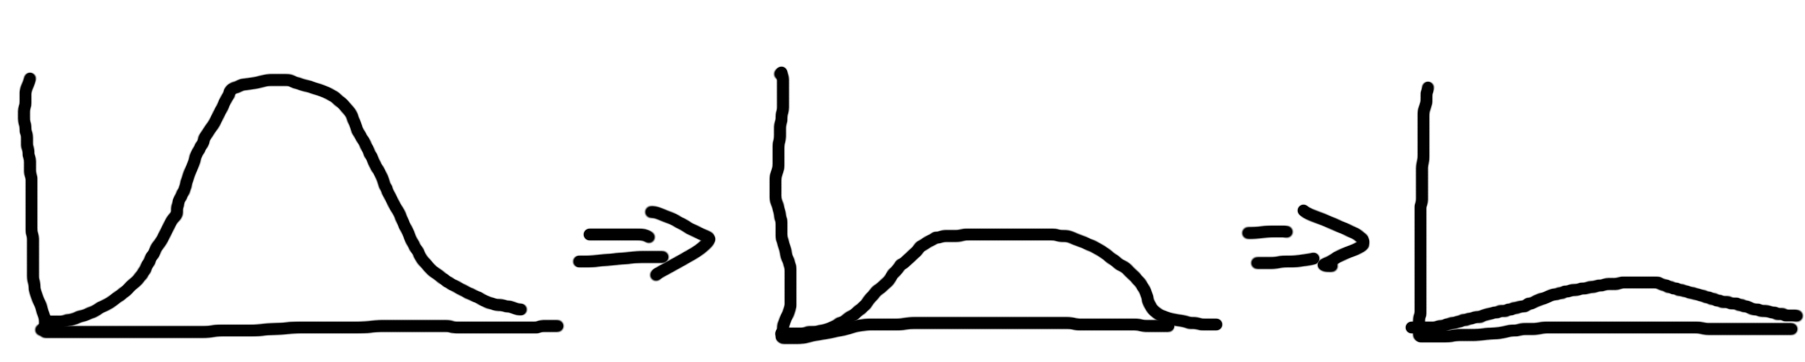
\includegraphics[scale=0.1]{Pictures/Dispersion.jpg}\\
$(\Delta x)^2(\Delta p)^2 = \frac{\hbar}{4}(1+\frac{a^2 t^2}{b^a}, a = \frac{1}{2}\frac{\partial^2\omega(k)}{\partial k^2}$
%
\subsection{Gebundene Zustände}
$\Psi(x,t)=\Psi(x,t)e^{\frac{-Et}{\hbar}}\Rightarrow \hat{H} \Psi(x,t)=E\Psi(x)$, mit Potential $\hat{H}=\frac{\hat{p}^2}{2m}+V(x)$\\
Falls V(x) stückweise konstant, löse:\\
$V(x)=V_1 x_1 \leq x < x_2, ---$\\
$\hat{H}\Psi(x)=(E-V_n)\Psi(x)$ Lösungen: $e^{ikx}, k =\pm\sqrt{\frac{2m(E-V_n}{\hbar^2}}$\\
%
\subsection{Randbedingungen}
$\Psi(x),\frac{\partial x\Psi(x)}{\Psi x} \in C^1$\\
%
\subsection{Streuzustände}
nicht normiert, ebene Wellen für $x\rightarrow \infty$  und/oder $x\rightarrow -\infty$\\
$\Psi(x)=e^{ikx}$, Amplitude 1\\
$\vec{j}=\frac{\hbar k}{m}=v_g, p = |\Psi|^2=1\Rightarrow j = p v_g = v_g$\\
Welche Anteile werden reflektiert (zurück gestreut) oder gehen weiter (vorwärts gestreut)\\
%
\subsection{Potential Barriere}
%
Breite a, für $x<a$ (I) und $x > a$ (III) $\Rightarrow V(x)=0$\\
$0\leq x$ (II) $\leq a \Rightarrow V(x)=V_0$\\
I+III: $k_1=k_3=\sqrt{\frac{2mE}{\hbar^2}}$ Wellenvektor\\
II: $k_2=\sqrt{\frac{2m(E-V_0}{\hbar}}, k \in \mathbb{R}$ falls $E>V_0$, sonst $k_2\in \mathbb{C}$\\
%
\\
$\Psi_I(x)=e^{ik_1x}+\underbrace{\gamma e^{-ik_1x}}_{Reflexieren}, \gamma = A+B-1$\\
$\Psi_{II}(x)=Ae^{ik_2x}+be^{ik_2x},A= \frac{te^{-ik_1x}}{2}(1+\frac{k_1}{k_2}),B=\frac{te^{ik_2x}}{2}(1+\frac{k_1}{k_2})$\\
$\Psi_{III}(x)=\underbrace{t}_{Transsmission}e^{ik_3(x-a)}$\\
%
\\
Für $E > V_0$\\
$|t|^2=\frac{UE(E-V_0)}{UE(E-V_0)+V_0^2\sin^2(k_2a)}$\\
%
\\
Für $E < V_0$\\
$|t|^2=\frac{UE(E-V_0)}{UE(E-V_0)+V_0^2\sinh^2(ka)}$\\
%
\\
mit: $k=\sqrt{\frac{2m(V_0-E}{\hbar}}$
\end{document}